\documentclass{standalone}
\usepackage{tikz}
\usetikzlibrary{patterns, positioning}
\usepackage[sfdefault]{ClearSans} %% option 'sfdefault' activates Clear Sans as the default text font
\usepackage[T1]{fontenc}

\begin{document}
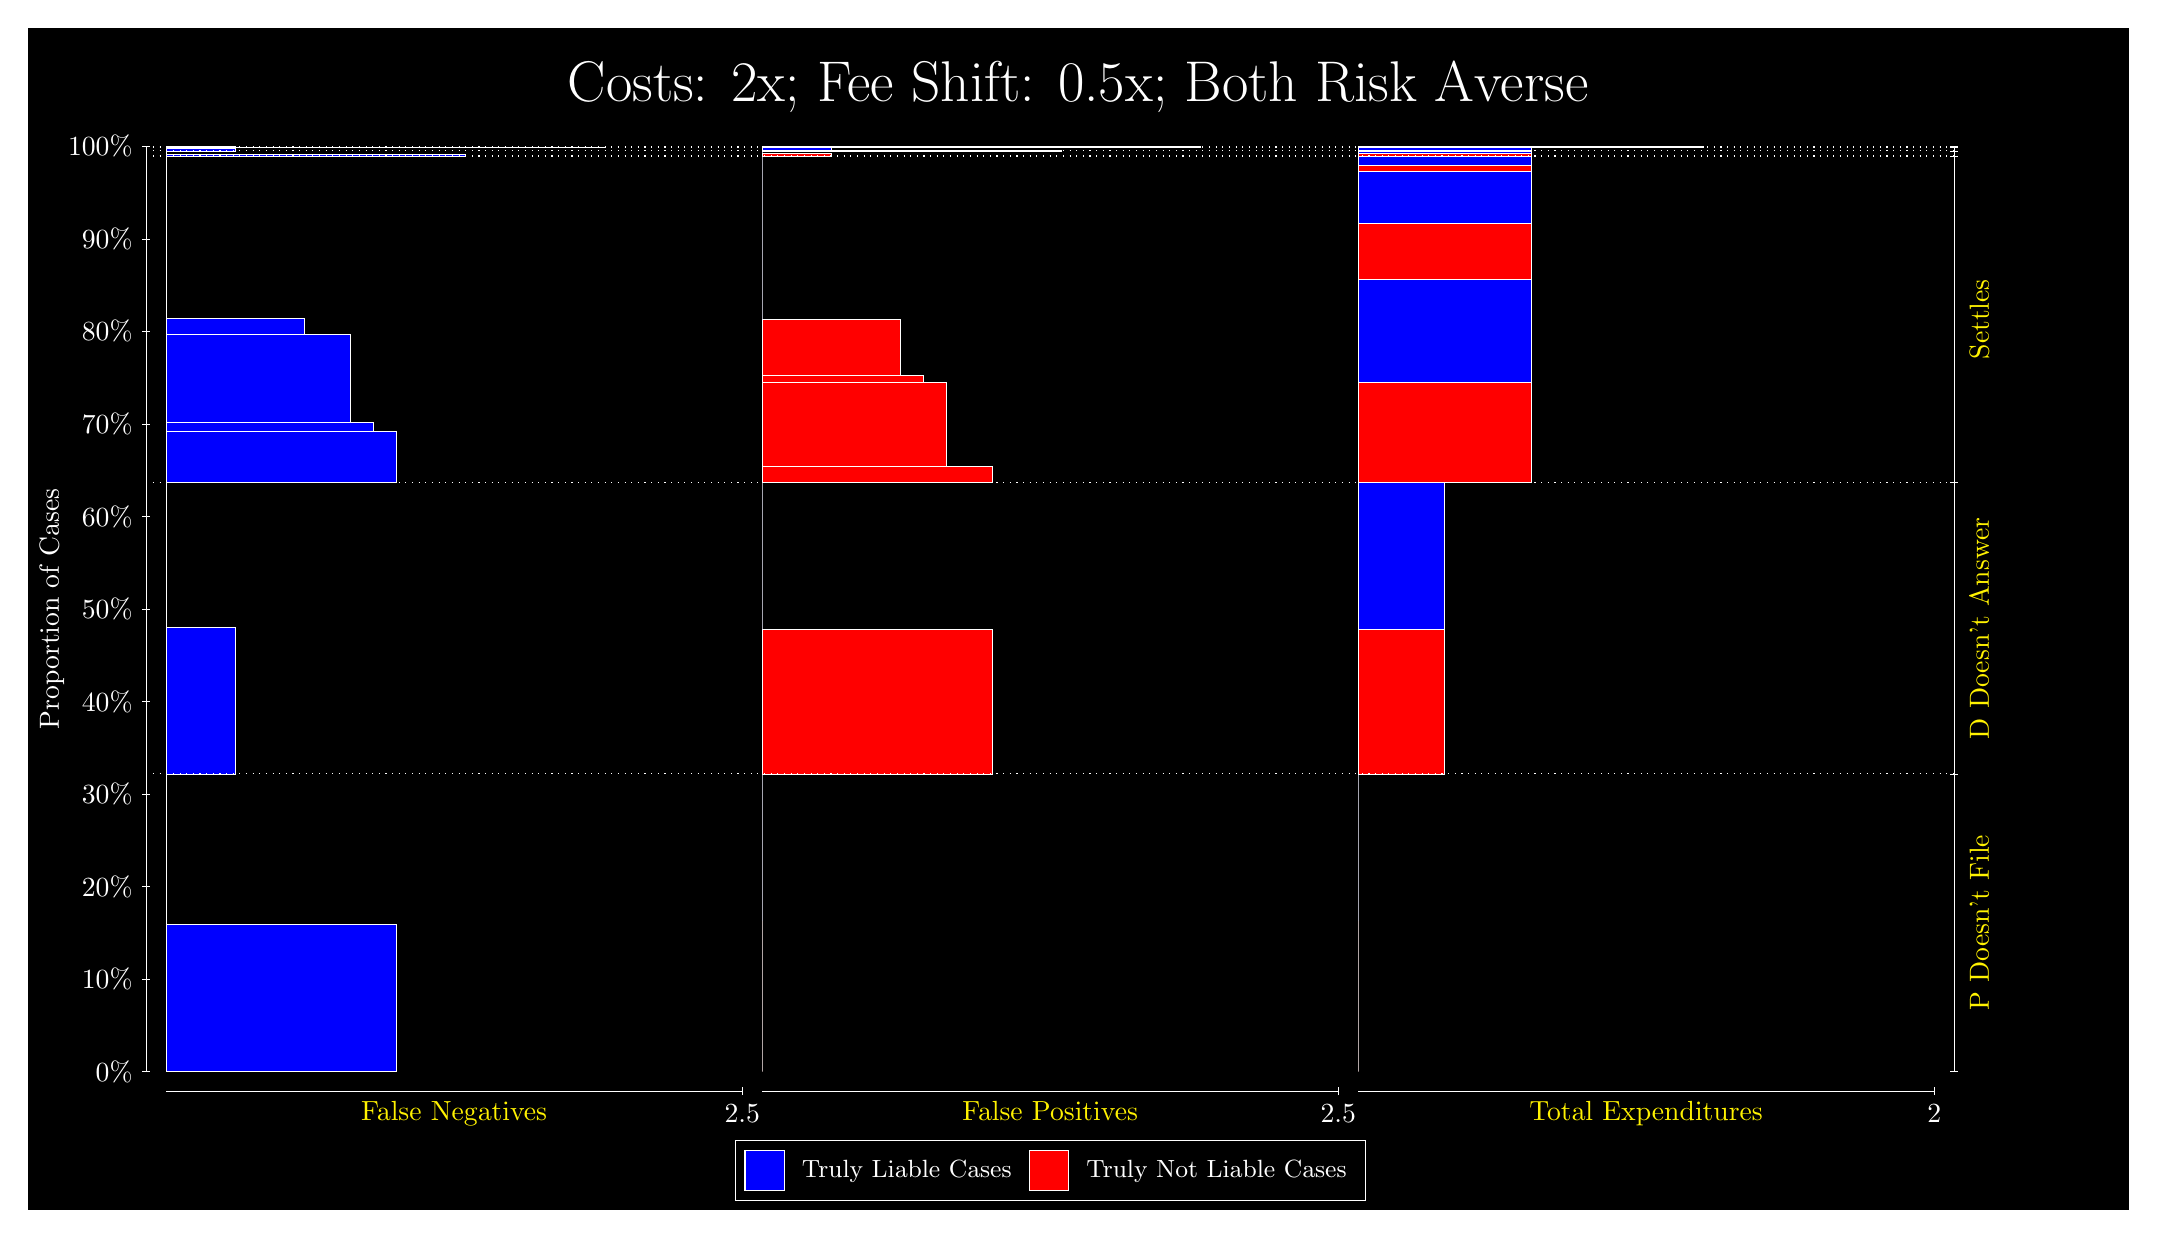
\begin{tikzpicture}
\draw[fill=black] (0,0) rectangle (26.667,15);
\draw[text=white] (0,13.5) rectangle (26.667,15) node[midway] {\huge Costs: 2x; Fee Shift: 0.5x; Both Risk Averse};
\draw[white, very thin] (1.5,1.75) -- (1.5,13.5);
\node[rotate=90, text=white, anchor=center] at (0.3, 7.625) {Proportion of Cases};
\draw[white, very thin] (1.45,1.75) -- (1.55,1.75);
\node[text=white, anchor=east] at (1.45, 1.75) {0\%};
\draw[white, very thin] (1.45,2.925) -- (1.55,2.925);
\node[text=white, anchor=east] at (1.45, 2.925) {10\%};
\draw[white, very thin] (1.45,4.1) -- (1.55,4.1);
\node[text=white, anchor=east] at (1.45, 4.1) {20\%};
\draw[white, very thin] (1.45,5.275) -- (1.55,5.275);
\node[text=white, anchor=east] at (1.45, 5.275) {30\%};
\draw[white, very thin] (1.45,6.45) -- (1.55,6.45);
\node[text=white, anchor=east] at (1.45, 6.45) {40\%};
\draw[white, very thin] (1.45,7.625) -- (1.55,7.625);
\node[text=white, anchor=east] at (1.45, 7.625) {50\%};
\draw[white, very thin] (1.45,8.8) -- (1.55,8.8);
\node[text=white, anchor=east] at (1.45, 8.8) {60\%};
\draw[white, very thin] (1.45,9.975) -- (1.55,9.975);
\node[text=white, anchor=east] at (1.45, 9.975) {70\%};
\draw[white, very thin] (1.45,11.15) -- (1.55,11.15);
\node[text=white, anchor=east] at (1.45, 11.15) {80\%};
\draw[white, very thin] (1.45,12.325) -- (1.55,12.325);
\node[text=white, anchor=east] at (1.45, 12.325) {90\%};
\draw[white, very thin] (1.45,13.5) -- (1.55,13.5);
\node[text=white, anchor=east] at (1.45, 13.5) {100\%};

\draw[white, very thin] (24.457,1.75) -- (24.457,13.5);
\draw[white, very thin] (24.407,1.75) -- (24.507,1.75);
\node[anchor=west] at (24.407, 1.75) {};
\draw[white, very thin] (24.407,5.5293) -- (24.507,5.5293);
\node[anchor=west] at (24.407, 5.5293) {};
\draw[white, very thin] (24.407,9.2302) -- (24.507,9.2302);
\node[anchor=west] at (24.407, 9.2302) {};
\draw[white, very thin] (24.407,13.377) -- (24.507,13.377);
\node[anchor=west] at (24.407, 13.377) {};
\draw[white, very thin] (24.407,13.442) -- (24.507,13.442);
\node[anchor=west] at (24.407, 13.442) {};
\draw[white, very thin] (24.407,13.485) -- (24.507,13.485);
\node[anchor=west] at (24.407, 13.485) {};
\draw[white, very thin] (24.407,13.492) -- (24.507,13.492);
\node[anchor=west] at (24.407, 13.492) {};
\draw[white, very thin] (24.407,13.5) -- (24.507,13.5);
\node[anchor=west] at (24.407, 13.5) {};

\draw[white, very thin, fill=blue] (1.75,1.75) rectangle (4.6775,3.6161);
\draw[white, very thin, fill=red] (1.75,3.6161) rectangle (1.75,5.5293);
\draw[white, very thin, fill=blue] (1.75,5.5293) rectangle (2.6283,7.3947);
\draw[white, very thin, fill=red] (1.75,7.3947) rectangle (1.75,9.2302);
\draw[white, very thin, fill=blue] (1.75,9.2302) rectangle (4.6775,9.886);
\draw[white, very thin, fill=blue] (1.75,9.886) rectangle (4.3848,9.9994);
\draw[white, very thin, fill=blue] (1.75,9.9994) rectangle (4.092,11.107);
\draw[white, very thin, fill=blue] (1.75,11.107) rectangle (3.5065,11.31);
\draw[white, very thin, fill=red] (1.75,11.31) rectangle (1.75,13.377);
\draw[white, very thin, fill=blue] (1.75,13.377) rectangle (5.5558,13.402);
\draw[white, very thin, fill=red] (1.75,13.402) rectangle (1.75,13.442);
\draw[white, very thin, fill=blue] (1.75,13.442) rectangle (2.6283,13.473);
\draw[white, very thin, fill=red] (1.75,13.473) rectangle (1.75,13.485);
\draw[white, very thin, fill=blue] (1.75,13.485) rectangle (7.3123,13.488);
\draw[white, very thin, fill=red] (1.75,13.488) rectangle (1.75,13.492);
\draw[white, very thin, fill=blue] (1.75,13.492) rectangle (2.6283,13.497);
\draw[white, very thin, fill=red] (1.75,13.497) rectangle (1.75,13.5);
\draw[white, very thin, fill=red] (9.3189,1.75) rectangle (9.3189,3.6632);
\draw[white, very thin, fill=blue] (9.3189,3.6632) rectangle (9.3189,5.5293);
\draw[white, very thin, fill=red] (9.3189,5.5293) rectangle (12.246,7.3648);
\draw[white, very thin, fill=blue] (9.3189,7.3648) rectangle (9.3189,9.2302);
\draw[white, very thin, fill=red] (9.3189,9.2302) rectangle (12.246,9.4328);
\draw[white, very thin, fill=red] (9.3189,9.4328) rectangle (11.661,10.503);
\draw[white, very thin, fill=red] (9.3189,10.503) rectangle (11.368,10.586);
\draw[white, very thin, fill=red] (9.3189,10.586) rectangle (11.075,11.298);
\draw[white, very thin, fill=blue] (9.3189,11.298) rectangle (9.3189,13.377);
\draw[white, very thin, fill=red] (9.3189,13.377) rectangle (10.197,13.417);
\draw[white, very thin, fill=blue] (9.3189,13.417) rectangle (9.3189,13.442);
\draw[white, very thin, fill=red] (9.3189,13.442) rectangle (13.125,13.454);
\draw[white, very thin, fill=blue] (9.3189,13.454) rectangle (10.197,13.485);
\draw[white, very thin, fill=red] (9.3189,13.485) rectangle (10.197,13.489);
\draw[white, very thin, fill=blue] (9.3189,13.489) rectangle (9.3189,13.492);
\draw[white, very thin, fill=red] (9.3189,13.492) rectangle (14.881,13.495);
\draw[white, very thin, fill=blue] (9.3189,13.495) rectangle (11.954,13.5);
\draw[white, very thin, fill=red] (16.888,1.75) rectangle (16.888,3.6632);
\draw[white, very thin, fill=blue] (16.888,3.6632) rectangle (16.888,5.5293);
\draw[white, very thin, fill=red] (16.888,5.5293) rectangle (17.986,7.3648);
\draw[white, very thin, fill=blue] (16.888,7.3648) rectangle (17.986,9.2302);
\draw[white, very thin, fill=red] (16.888,9.2302) rectangle (19.083,10.503);
\draw[white, very thin, fill=blue] (16.888,10.503) rectangle (19.083,11.813);
\draw[white, very thin, fill=red] (16.888,11.813) rectangle (19.083,12.525);
\draw[white, very thin, fill=blue] (16.888,12.525) rectangle (19.083,13.181);
\draw[white, very thin, fill=red] (16.888,13.181) rectangle (19.083,13.264);
\draw[white, very thin, fill=blue] (16.888,13.264) rectangle (19.083,13.377);
\draw[white, very thin, fill=red] (16.888,13.377) rectangle (19.083,13.417);
\draw[white, very thin, fill=blue] (16.888,13.417) rectangle (19.083,13.442);
\draw[white, very thin, fill=red] (16.888,13.442) rectangle (19.083,13.454);
\draw[white, very thin, fill=blue] (16.888,13.454) rectangle (19.083,13.485);
\draw[white, very thin, fill=red] (16.888,13.485) rectangle (21.279,13.489);
\draw[white, very thin, fill=blue] (16.888,13.489) rectangle (21.279,13.492);
\draw[white, very thin, fill=red] (16.888,13.492) rectangle (21.279,13.495);
\draw[white, very thin, fill=blue] (16.888,13.495) rectangle (21.279,13.5);
\draw[white, dotted] (1.5,5.5293) -- (24.457,5.5293);
\draw[white, dotted] (1.5,9.2302) -- (24.457,9.2302);
\draw[white, dotted] (1.5,13.377) -- (24.457,13.377);
\draw[white, dotted] (1.5,13.442) -- (24.457,13.442);
\draw[white, dotted] (1.5,13.485) -- (24.457,13.485);
\draw[white, dotted] (1.5,13.492) -- (24.457,13.492);
\draw[white, very thin] (1.75,1.5) -- (9.0689,1.5);
\node[text=yellow, anchor=north] at (5.4094, 1.5) {False Negatives};
\draw[white, very thin] (9.0689,1.45) -- (9.0689,1.55);
\node[text=white, anchor=north] at (9.0689, 1.45) {2.5};

\draw[white, very thin] (9.3189,1.5) -- (16.638,1.5);
\node[text=yellow, anchor=north] at (12.978, 1.5) {False Positives};
\draw[white, very thin] (16.638,1.45) -- (16.638,1.55);
\node[text=white, anchor=north] at (16.638, 1.45) {2.5};

\draw[white, very thin] (16.888,1.5) -- (24.207,1.5);
\node[text=yellow, anchor=north] at (20.547, 1.5) {Total Expenditures};
\draw[white, very thin] (24.207,1.45) -- (24.207,1.55);
\node[text=white, anchor=north] at (24.207, 1.45) {2};

\node[text=yellow, centered, rotate=90] at (24.777, 3.6396) {P Doesn't File};
\node[text=yellow, centered, rotate=90] at (24.777, 7.3797) {D Doesn't Answer};
\node[text=yellow, centered, rotate=90] at (24.777, 11.304) {Settles};





\draw (12.978300999999998,1.5) node[draw=none] (baseCoordinate) {};
\begin{scope}[align=center]
        \matrix[scale=0.5, draw=white, below=0.5cm of baseCoordinate, nodes={draw}, column sep=0.1cm]{
            \node[rectangle, draw, minimum width=0.5cm, minimum height=0.5cm, fill=blue] {}; &
            \node[draw=none, font=\small, text=white] (B) {Truly Liable Cases}; &
            \node[rectangle, draw, minimum width=0.5cm, minimum height=0.5cm, fill=red] {}; &
            \node[draw=none, font=\small, text=white] (B) {Truly Not Liable Cases}; \\
            };
\end{scope}

\end{tikzpicture}
\end{document}